\chapter{Memory}\label{memory}

A solid understanding of R's memory management will help you predict how
much memory you'll need for a given task and help you to make the most
of the memory you have. It can even help you write faster code because
accidental copies are a major cause of slow code. The goal of this
chapter is to help you understand the basics of memory management in R,
moving from individual objects to functions to larger blocks of code.
Along the way, you'll learn about some common myths, such as that you
need to call \texttt{gc()} to free up memory, or that \texttt{for} loops
are always slow. \index{memory}

\paragraph{Outline}

\begin{itemize}
\item
  \hyperref[object-size]{Object size} shows you how to use
  \texttt{object\_size()} to see how much memory an object occupies, and
  uses that as a launching point to improve your understanding of how R
  objects are stored in memory.
\item
  \hyperref[gc]{Memory usage and garbage collection} introduces you to
  the \texttt{mem\_used()} and \texttt{mem\_changed()} functions that
  will help you understand how R allocates and frees memory.
\item
  \hyperref[memory-profiling]{Memory profiling with lineprof} shows you
  how to use the lineprof package to understand how memory is allocated
  and released in larger code blocks.
\item
  \hyperref[modification]{Modification in place} introduces you to the
  \texttt{address()} and \texttt{refs()} functions so that you can
  understand when R modifies in place and when R modifies a copy.
  Understanding when objects are copied is very important for writing
  efficient R code.
\end{itemize}

\paragraph{Prerequisites}

In this chapter, we'll use tools from the pryr and lineprof packages to
understand memory usage, and a sample dataset from ggplot2. If you don't
already have them, run this code to get the packages you need:

\begin{Shaded}
\begin{Highlighting}[]
\KeywordTok{install.packages}\NormalTok{(}\StringTok{"ggplot2"}\NormalTok{)}
\KeywordTok{install.packages}\NormalTok{(}\StringTok{"pryr"}\NormalTok{)}
\NormalTok{devtools::}\KeywordTok{install_github}\NormalTok{(}\StringTok{"hadley/lineprof"}\NormalTok{)}
\end{Highlighting}
\end{Shaded}

\paragraph{Sources}

The details of R's memory management are not documented in a single
place. Most of the information in this chapter was gleaned from a close
reading of the documentation (particularly \texttt{?Memory} and
\texttt{?gc}), the
\href{http://cran.r-project.org/doc/manuals/R-exts.html\#Profiling-R-code-for-memory-use}{memory
profiling} section of R-exts, and the
\href{http://cran.r-project.org/doc/manuals/R-ints.html\#SEXPs}{SEXPs}
section of R-ints. The rest I figured out by reading the C source code,
performing small experiments, and asking questions on R-devel. Any
mistakes are entirely mine.

\hyperdef{}{object-size}{\section{Object size}\label{object-size}}

To understand memory usage in R, we will start with
\texttt{pryr::object\_size()}. This function tells you how many bytes of
memory an object occupies: \index{object\_size()}

\begin{Shaded}
\begin{Highlighting}[]
\KeywordTok{library}\NormalTok{(pryr)}
\KeywordTok{object_size}\NormalTok{(}\DecValTok{1}\NormalTok{:}\DecValTok{10}\NormalTok{)}
\CommentTok{#> 88 B}
\KeywordTok{object_size}\NormalTok{(mean)}
\CommentTok{#> 832 B}
\KeywordTok{object_size}\NormalTok{(mtcars)}
\CommentTok{#> 6.74 kB}
\end{Highlighting}
\end{Shaded}

(This function is better than the built-in \texttt{object.size()}
because it accounts for shared elements within an object and includes
the size of environments.)

Something interesting occurs if we use \texttt{object\_size()} to
systematically explore the size of an integer vector. The code below
computes and plots the memory usage of integer vectors ranging in length
from 0 to 50 elements. You might expect that the size of an empty vector
would be zero and that memory usage would grow proportionately with
length. Neither of those things are true! \index{vectors!size of}

\begin{Shaded}
\begin{Highlighting}[]
\NormalTok{sizes <-}\StringTok{ }\KeywordTok{sapply}\NormalTok{(}\DecValTok{0}\NormalTok{:}\DecValTok{50}\NormalTok{, function(n) }\KeywordTok{object_size}\NormalTok{(}\KeywordTok{seq_len}\NormalTok{(n)))}
\KeywordTok{plot}\NormalTok{(}\DecValTok{0}\NormalTok{:}\DecValTok{50}\NormalTok{, sizes, }\DataTypeTok{xlab =} \StringTok{"Length"}\NormalTok{, }\DataTypeTok{ylab =} \StringTok{"Size (bytes)"}\NormalTok{, }
  \DataTypeTok{type =} \StringTok{"s"}\NormalTok{)}
\end{Highlighting}
\end{Shaded}

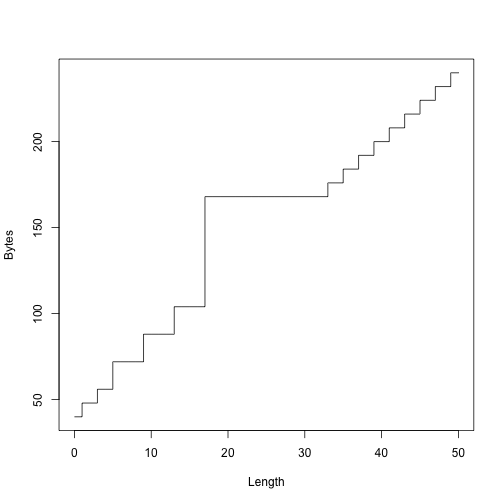
\includegraphics{figures/size-q.pdf}

This isn't just an artefact of integer vectors. Every length 0 vector
occupies 40 bytes of memory:

\begin{Shaded}
\begin{Highlighting}[]
\KeywordTok{object_size}\NormalTok{(}\KeywordTok{numeric}\NormalTok{())}
\CommentTok{#> 40 B}
\KeywordTok{object_size}\NormalTok{(}\KeywordTok{logical}\NormalTok{())}
\CommentTok{#> 40 B}
\KeywordTok{object_size}\NormalTok{(}\KeywordTok{raw}\NormalTok{())}
\CommentTok{#> 40 B}
\KeywordTok{object_size}\NormalTok{(}\KeywordTok{list}\NormalTok{())}
\CommentTok{#> 40 B}
\end{Highlighting}
\end{Shaded}

Those 40 bytes are used to store four components possessed by every
object in R:

\begin{itemize}
\item
  Object metadata (4 bytes). These metadata store the base type
  (e.g.~integer) and information used for debugging and memory
  management.
\item
  Two pointers: one to the next object in memory and one to the previous
  object (2 * 8 bytes). This doubly-linked list makes it easy for
  internal R code to loop through every object in memory.
\item
  A pointer to the attributes (8 bytes).
\end{itemize}

All vectors have three additional components: \indexc{SEXP}

\begin{itemize}
\item
  The length of the vector (4 bytes). By using only 4 bytes, you might
  expect that R could only support vectors up to $2 ^ {4 \times 8 - 1}$
  ($2 ^ {31}$, about two billion) elements. But in R 3.0.0 and later,
  you can actually have vectors up to $2 ^ {52}$ elements.
  \href{http://cran.r-project.org/doc/manuals/R-ints.html\#Long-vectors}{Read
  R-internals} to see how support for long vectors was added without
  having to change the size of this field. \index{long vectors}
  \index{atomic vectors!long}
\item
  The ``true'' length of the vector (4 bytes). This is basically never
  used, except when the object is the hash table used for an
  environment. In that case, the true length represents the allocated
  space, and the length represents the space currently used.
\item
  The data (?? bytes). An empty vector has 0 bytes of data, but it's
  obviously very important otherwise! Numeric vectors occupy 8 bytes for
  every element, integer vectors 4, and complex vectors 16.
\end{itemize}

If you're keeping count you'll notice that this only adds up to 36
bytes. The remaining 4 bytes are used for padding so that each component
starts on an 8 byte (= 64-bit) boundary. Most cpu architectures require
pointers to be aligned in this way, and even if they don't require it,
accessing non-aligned pointers tends to be rather slow. (If you're
interested, you can read more about it in
\href{http://www.catb.org/esr/structure-packing/}{C structure packing}.)

This explains the intercept on the graph. But why does the memory size
grow irregularly? To understand why, you need to know a little bit about
how R requests memory from the operating system. Requesting memory (with
\texttt{malloc()}) is a relatively expensive operation. Having to
request memory every time a small vector is created would slow R down
considerably. Instead, R asks for a big block of memory and then manages
that block itself. This block is called the small vector pool and is
used for vectors less than 128 bytes long. For efficiency and
simplicity, it only allocates vectors that are 8, 16, 32, 48, 64, or 128
bytes long. If we adjust our previous plot to remove the 40 bytes of
overhead, we can see that those values correspond to the jumps in memory
use.

\begin{Shaded}
\begin{Highlighting}[]
\KeywordTok{plot}\NormalTok{(}\DecValTok{0}\NormalTok{:}\DecValTok{50}\NormalTok{, sizes -}\StringTok{ }\DecValTok{40}\NormalTok{, }\DataTypeTok{xlab =} \StringTok{"Length"}\NormalTok{, }
  \DataTypeTok{ylab =} \StringTok{"Bytes excluding overhead"}\NormalTok{, }\DataTypeTok{type =} \StringTok{"n"}\NormalTok{)}
\KeywordTok{abline}\NormalTok{(}\DataTypeTok{h =} \DecValTok{0}\NormalTok{, }\DataTypeTok{col =} \StringTok{"grey80"}\NormalTok{)}
\KeywordTok{abline}\NormalTok{(}\DataTypeTok{h =} \KeywordTok{c}\NormalTok{(}\DecValTok{8}\NormalTok{, }\DecValTok{16}\NormalTok{, }\DecValTok{32}\NormalTok{, }\DecValTok{48}\NormalTok{, }\DecValTok{64}\NormalTok{, }\DecValTok{128}\NormalTok{), }\DataTypeTok{col =} \StringTok{"grey80"}\NormalTok{)}
\KeywordTok{abline}\NormalTok{(}\DataTypeTok{a =} \DecValTok{0}\NormalTok{, }\DataTypeTok{b =} \DecValTok{4}\NormalTok{, }\DataTypeTok{col =} \StringTok{"grey90"}\NormalTok{, }\DataTypeTok{lwd =} \DecValTok{4}\NormalTok{)}
\KeywordTok{lines}\NormalTok{(sizes -}\StringTok{ }\DecValTok{40}\NormalTok{, }\DataTypeTok{type =} \StringTok{"s"}\NormalTok{)}
\end{Highlighting}
\end{Shaded}

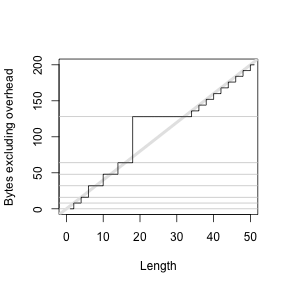
\includegraphics{figures/size-a.pdf}

Beyond 128 bytes, it no longer makes sense for R to manage vectors.
After all, allocating big chunks of memory is something that operating
systems are very good at. Beyond 128 bytes, R will ask for memory in
multiples of 8 bytes. This ensures good alignment.

A subtlety of the size of an object is that components can be shared
across multiple objects. For example, look at the following code:

\begin{Shaded}
\begin{Highlighting}[]
\NormalTok{x <-}\StringTok{ }\DecValTok{1}\NormalTok{:}\FloatTok{1e6}
\KeywordTok{object_size}\NormalTok{(x)}
\CommentTok{#> 4 MB}

\NormalTok{y <-}\StringTok{ }\KeywordTok{list}\NormalTok{(x, x, x)}
\KeywordTok{object_size}\NormalTok{(y)}
\CommentTok{#> 4 MB}
\end{Highlighting}
\end{Shaded}

\texttt{y} isn't three times as big as \texttt{x} because R is smart
enough to not copy \texttt{x} three times; instead it just points to the
existing \texttt{x}.

It's misleading to look at the sizes of \texttt{x} and \texttt{y}
individually. If you want to know how much space they take up together,
you have to supply them to the same \texttt{object\_size()} call:

\begin{Shaded}
\begin{Highlighting}[]
\KeywordTok{object_size}\NormalTok{(x, y)}
\CommentTok{#> 4 MB}
\end{Highlighting}
\end{Shaded}

In this case, \texttt{x} and \texttt{y} together take up the same amount
of space as \texttt{y} alone. This is not always the case. If there are
no shared components, as in the following example, then you can add up
the sizes of individual components to find out the total size:

\begin{Shaded}
\begin{Highlighting}[]
\NormalTok{x1 <-}\StringTok{ }\DecValTok{1}\NormalTok{:}\FloatTok{1e6}
\NormalTok{y1 <-}\StringTok{ }\KeywordTok{list}\NormalTok{(}\DecValTok{1}\NormalTok{:}\FloatTok{1e6}\NormalTok{, }\DecValTok{1}\NormalTok{:}\FloatTok{1e6}\NormalTok{, }\DecValTok{1}\NormalTok{:}\FloatTok{1e6}\NormalTok{)}

\KeywordTok{object_size}\NormalTok{(x1)}
\CommentTok{#> 4 MB}
\KeywordTok{object_size}\NormalTok{(y1)}
\CommentTok{#> 12 MB}
\KeywordTok{object_size}\NormalTok{(x1, y1)}
\CommentTok{#> 16 MB}
\KeywordTok{object_size}\NormalTok{(x1) +}\StringTok{ }\KeywordTok{object_size}\NormalTok{(y1) ==}\StringTok{ }\KeywordTok{object_size}\NormalTok{(x1, y1)}
\CommentTok{#> [1] TRUE}
\end{Highlighting}
\end{Shaded}

The same issue also comes up with strings, because R has a global string
pool. This means that each unique string is only stored in one place,
and therefore character vectors take up less memory than you might
expect: \index{string pool}

\begin{Shaded}
\begin{Highlighting}[]
\KeywordTok{object_size}\NormalTok{(}\StringTok{"banana"}\NormalTok{)}
\CommentTok{#> 96 B}
\KeywordTok{object_size}\NormalTok{(}\KeywordTok{rep}\NormalTok{(}\StringTok{"banana"}\NormalTok{, }\DecValTok{10}\NormalTok{))}
\CommentTok{#> 216 B}
\end{Highlighting}
\end{Shaded}

\subsection{Exercises}

\begin{enumerate}
\def\labelenumi{\arabic{enumi}.}
\item
  Repeat the analysis above for numeric, logical, and complex vectors.
\item
  If a data frame has one million rows, and three variables (two
  numeric, and one integer), how much space will it take up? Work out it
  out from theory, then verify your work by creating a data frame and
  measuring its size.
\item
  Compare the sizes of the elements in the following two lists. Each
  contains basically the same data, but one contains vectors of small
  strings while the other contains a single long string.

\begin{Shaded}
\begin{Highlighting}[]
\NormalTok{vec <-}\StringTok{ }\KeywordTok{lapply}\NormalTok{(}\DecValTok{0}\NormalTok{:}\DecValTok{50}\NormalTok{, function(i) }\KeywordTok{c}\NormalTok{(}\StringTok{"ba"}\NormalTok{, }\KeywordTok{rep}\NormalTok{(}\StringTok{"na"}\NormalTok{, i)))}
\NormalTok{str <-}\StringTok{ }\KeywordTok{lapply}\NormalTok{(vec, paste0, }\DataTypeTok{collapse =} \StringTok{""}\NormalTok{)}
\end{Highlighting}
\end{Shaded}
\item
  Which takes up more memory: a factor (\texttt{x}) or the equivalent
  character vector (\texttt{as.character(x)})? Why?
\item
  Explain the difference in size between \texttt{1:5} and
  \texttt{list(1:5)}.
\end{enumerate}

\hyperdef{}{gc}{\section{Memory usage and garbage collection}\label{gc}}

While \texttt{object\_size()} tells you the size of a single object,
\texttt{pryr::mem\_used()} tells you the total size of all objects in
memory: \indexc{mem\_used()}

\begin{Shaded}
\begin{Highlighting}[]
\KeywordTok{library}\NormalTok{(pryr)}
\KeywordTok{mem_used}\NormalTok{()}
\CommentTok{#> 45.4 MB}
\end{Highlighting}
\end{Shaded}

This number won't agree with the amount of memory reported by your
operating system for a number of reasons:

\begin{enumerate}
\def\labelenumi{\arabic{enumi}.}
\item
  It only includes objects created by R, not the R interpreter itself.
\item
  Both R and the operating system are lazy: they won't reclaim memory
  until it's actually needed. R might be holding on to memory because
  the OS hasn't yet asked for it back.
\item
  R counts the memory occupied by objects but there may be gaps due to
  deleted objects. This problem is known as memory fragmentation.
\end{enumerate}

\texttt{mem\_change()} builds on top of \texttt{mem\_used()} to tell you
how memory changes during code execution. Positive numbers represent an
increase in the memory used by R, and negative numbers represent a
decrease. \indexc{mem\_change()}

\begin{Shaded}
\begin{Highlighting}[]
\CommentTok{# Need about 4 mb to store 1 million integers}
\KeywordTok{mem_change}\NormalTok{(x <-}\StringTok{ }\DecValTok{1}\NormalTok{:}\FloatTok{1e6}\NormalTok{)}
\CommentTok{#> 4.01 MB}
\CommentTok{# We get that memory back when we delete it}
\KeywordTok{mem_change}\NormalTok{(}\KeywordTok{rm}\NormalTok{(x))}
\CommentTok{#> -4 MB}
\end{Highlighting}
\end{Shaded}

Even operations that don't do anything use up a little memory. This is
because R is tracking the history of everything you do. You can ignore
anything on the order of around 2 kB.

\begin{Shaded}
\begin{Highlighting}[]
\KeywordTok{mem_change}\NormalTok{(}\OtherTok{NULL}\NormalTok{)}
\CommentTok{#> 1.47 kB}
\KeywordTok{mem_change}\NormalTok{(}\OtherTok{NULL}\NormalTok{)}
\CommentTok{#> 1.47 kB}
\end{Highlighting}
\end{Shaded}

In some languages, you have to explicitly delete unused objects for
their memory to be returned. R uses an alternative approach: garbage
collection (or GC for short). GC automatically releases memory when an
object is no longer used. It does this by tracking how many names point
to each object, and when there are no names pointing to an object, it
deletes that object. \index{garbage collection}

\begin{Shaded}
\begin{Highlighting}[]
\CommentTok{# Create a big object}
\KeywordTok{mem_change}\NormalTok{(x <-}\StringTok{ }\DecValTok{1}\NormalTok{:}\FloatTok{1e6}\NormalTok{)}
\CommentTok{#> 4 MB}
\CommentTok{# Also point to 1:1e6 from y}
\KeywordTok{mem_change}\NormalTok{(y <-}\StringTok{ }\NormalTok{x)}
\CommentTok{#> -4 MB}
\CommentTok{# Remove x, no memory freed because y is still pointing to it}
\KeywordTok{mem_change}\NormalTok{(}\KeywordTok{rm}\NormalTok{(x))}
\CommentTok{#> 1.42 kB}
\CommentTok{# Now nothing points to it and the memory can be freed}
\KeywordTok{mem_change}\NormalTok{(}\KeywordTok{rm}\NormalTok{(y))}
\CommentTok{#> -4 MB}
\end{Highlighting}
\end{Shaded}

Despite what you might have read elsewhere, there's never any need to
call \texttt{gc()} yourself. R will automatically run garbage collection
whenever it needs more space; if you want to see when that is, call
\texttt{gcinfo(TRUE)}. The only reason you \emph{might} want to call
\texttt{gc()} is to ask R to return memory to the operating system.
However, even that might not have any effect: older versions of Windows
had no way for a program to return memory to the OS. \indexc{gc()}

GC takes care of releasing objects that are no longer used. However, you
do need to be aware of possible memory leaks. A memory leak occurs when
you keep pointing to an object without realising it. In R, the two main
causes of memory leaks are formulas and closures because they both
capture the enclosing environment. The following code illustrates the
problem. In \texttt{f1()}, \texttt{1:1e6} is only referenced inside the
function, so when the function completes the memory is returned and the
net change is 0. The net memory change will be 0. \texttt{f2()} and
\texttt{f3()} both return objects that capture environments, so that
\texttt{x} is not freed when the function completes.
\index{memory!leaks}

\begin{Shaded}
\begin{Highlighting}[]
\NormalTok{f1 <-}\StringTok{ }\NormalTok{function() \{}
  \NormalTok{x <-}\StringTok{ }\DecValTok{1}\NormalTok{:}\FloatTok{1e6}
  \DecValTok{10}
\NormalTok{\}}
\KeywordTok{mem_change}\NormalTok{(x <-}\StringTok{ }\KeywordTok{f1}\NormalTok{())}
\CommentTok{#> 1.38 kB}
\KeywordTok{object_size}\NormalTok{(x)}
\CommentTok{#> 48 B}

\NormalTok{f2 <-}\StringTok{ }\NormalTok{function() \{}
  \NormalTok{x <-}\StringTok{ }\DecValTok{1}\NormalTok{:}\FloatTok{1e6}
  \NormalTok{a ~}\StringTok{ }\NormalTok{b}
\NormalTok{\}}
\KeywordTok{mem_change}\NormalTok{(y <-}\StringTok{ }\KeywordTok{f2}\NormalTok{())}
\CommentTok{#> 4 MB}
\KeywordTok{object_size}\NormalTok{(y)}
\CommentTok{#> 4 MB}

\NormalTok{f3 <-}\StringTok{ }\NormalTok{function() \{}
  \NormalTok{x <-}\StringTok{ }\DecValTok{1}\NormalTok{:}\FloatTok{1e6}
  \NormalTok{function() }\DecValTok{10}
\NormalTok{\}}
\KeywordTok{mem_change}\NormalTok{(z <-}\StringTok{ }\KeywordTok{f3}\NormalTok{())}
\CommentTok{#> 4 MB}
\KeywordTok{object_size}\NormalTok{(z)}
\CommentTok{#> 4.01 MB}
\end{Highlighting}
\end{Shaded}

\hyperdef{}{memory-profiling}{\section{Memory profiling with
lineprof}\label{memory-profiling}}

\texttt{mem\_change()} captures the net change in memory when running a
block of code. Sometimes, however, we may want to measure incremental
change. One way to do this is to use memory profiling to capture usage
every few milliseconds. This functionality is provided by
\texttt{utils::Rprof()} but it doesn't provide a very useful display of
the results. Instead we'll use the
\href{https://github.com/hadley/lineprof}{lineprof} package. It is
powered by \texttt{Rprof()}, but displays the results in a more
informative manner. \index{memory!profiling}

To demonstrate \texttt{lineprof}, we're going to explore a bare-bones
implementation of \texttt{read.delim()} with only three arguments:
\indexc{read\_delim()}

\begin{Shaded}
\begin{Highlighting}[]
\NormalTok{read_delim <-}\StringTok{ }\NormalTok{function(file, }\DataTypeTok{header =} \OtherTok{TRUE}\NormalTok{, }\DataTypeTok{sep =} \StringTok{","}\NormalTok{) \{}
  \CommentTok{# Determine number of fields by reading first line}
  \NormalTok{first <-}\StringTok{ }\KeywordTok{scan}\NormalTok{(file, }\DataTypeTok{what =} \KeywordTok{character}\NormalTok{(}\DecValTok{1}\NormalTok{), }\DataTypeTok{nlines =} \DecValTok{1}\NormalTok{,}
    \DataTypeTok{sep =} \NormalTok{sep, }\DataTypeTok{quiet =} \OtherTok{TRUE}\NormalTok{)}
  \NormalTok{p <-}\StringTok{ }\KeywordTok{length}\NormalTok{(first)}

  \CommentTok{# Load all fields as character vectors}
  \NormalTok{all <-}\StringTok{ }\KeywordTok{scan}\NormalTok{(file, }\DataTypeTok{what =} \KeywordTok{as.list}\NormalTok{(}\KeywordTok{rep}\NormalTok{(}\StringTok{"character"}\NormalTok{, p)),}
    \DataTypeTok{sep =} \NormalTok{sep, }\DataTypeTok{skip =} \NormalTok{if (header) }\DecValTok{1} \NormalTok{else }\DecValTok{0}\NormalTok{, }\DataTypeTok{quiet =} \OtherTok{TRUE}\NormalTok{)}

  \CommentTok{# Convert from strings to appropriate types (never to factors)}
  \NormalTok{all[] <-}\StringTok{ }\KeywordTok{lapply}\NormalTok{(all, type.convert, }\DataTypeTok{as.is =} \OtherTok{TRUE}\NormalTok{)}

  \CommentTok{# Set column names}
  \NormalTok{if (header) \{}
    \KeywordTok{names}\NormalTok{(all) <-}\StringTok{ }\NormalTok{first}
  \NormalTok{\} else \{}
    \KeywordTok{names}\NormalTok{(all) <-}\StringTok{ }\KeywordTok{paste0}\NormalTok{(}\StringTok{"V"}\NormalTok{, }\KeywordTok{seq_along}\NormalTok{(all))}
  \NormalTok{\}}

  \CommentTok{# Convert list into data frame}
  \KeywordTok{as.data.frame}\NormalTok{(all)}
\NormalTok{\}}
\end{Highlighting}
\end{Shaded}

We'll also create a sample csv file:

\begin{Shaded}
\begin{Highlighting}[]
\KeywordTok{library}\NormalTok{(ggplot2)}
\KeywordTok{write.csv}\NormalTok{(diamonds, }\StringTok{"diamonds.csv"}\NormalTok{, }\DataTypeTok{row.names =} \OtherTok{FALSE}\NormalTok{)}
\end{Highlighting}
\end{Shaded}

Using lineprof is straightforward. \texttt{source()} the code, apply
\texttt{lineprof()} to an expression, then use \texttt{shine()} to view
the results. Note that you \emph{must} use \texttt{source()} to load the
code. This is because lineprof uses srcrefs to match up the code and run
times. The needed srcrefs are only created when you load code from disk.

\begin{Shaded}
\begin{Highlighting}[]
\KeywordTok{library}\NormalTok{(lineprof)}

\KeywordTok{source}\NormalTok{(}\StringTok{"code/read-delim.R"}\NormalTok{)}
\NormalTok{prof <-}\StringTok{ }\KeywordTok{lineprof}\NormalTok{(}\KeywordTok{read_delim}\NormalTok{(}\StringTok{"diamonds.csv"}\NormalTok{))}
\KeywordTok{shine}\NormalTok{(prof)}
\end{Highlighting}
\end{Shaded}

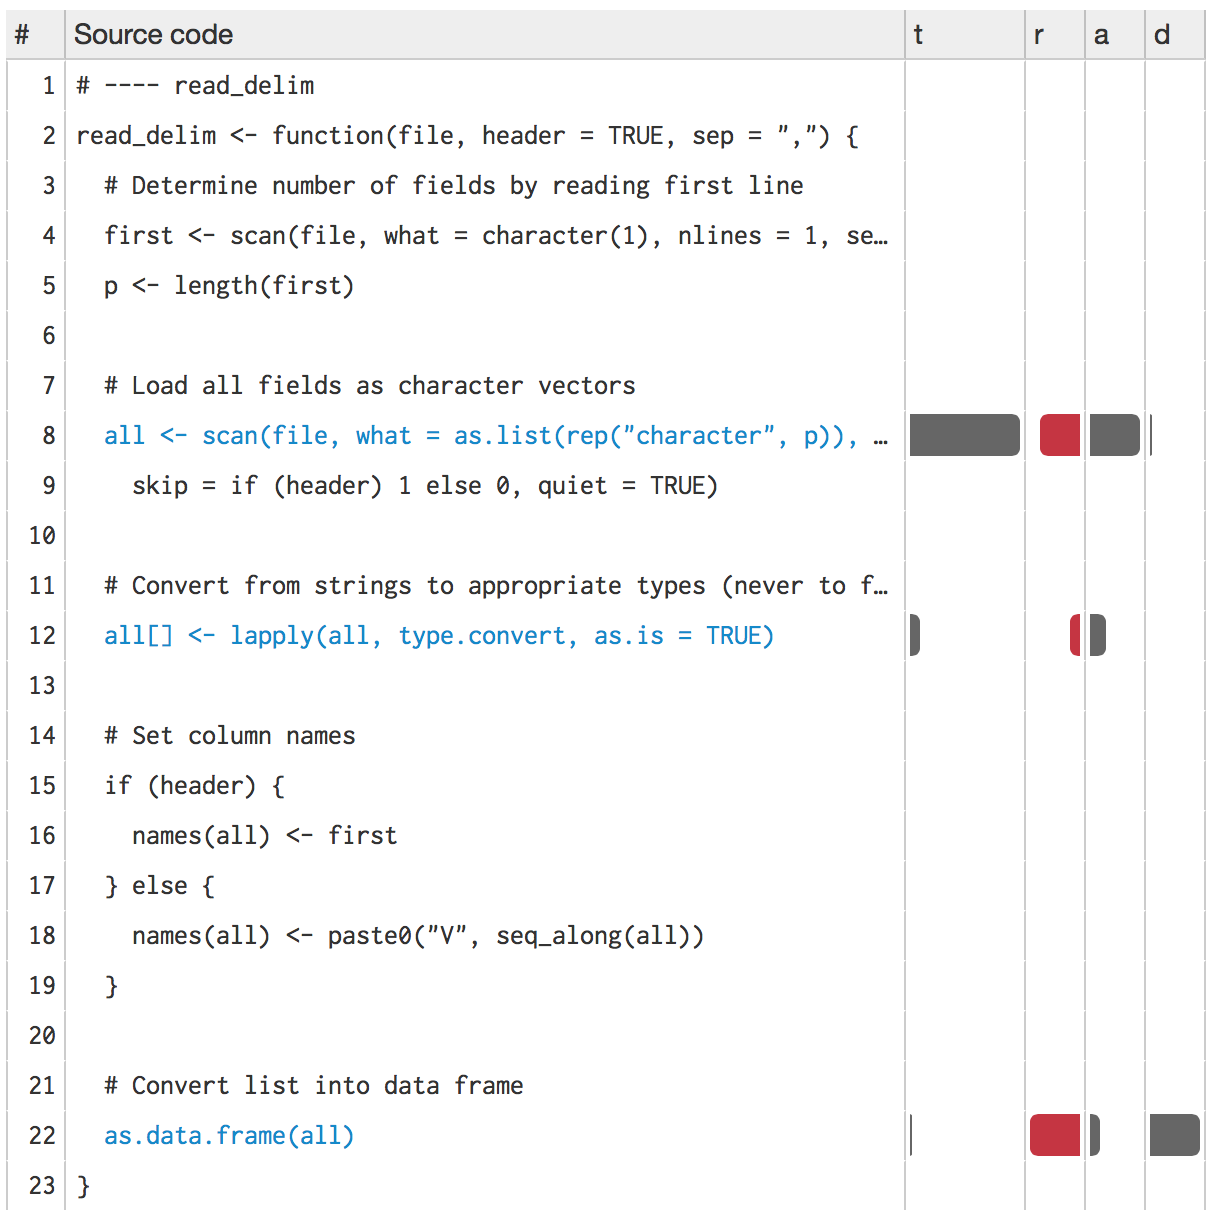
\includegraphics[width=4.35in]{screenshots/memory-lineprof.png}

\texttt{shine()} will also open a new web page (or if you're using
RStudio, a new pane) that shows your source code annotated with
information about memory usage. \texttt{shine()} starts a shiny app
which will ``block'' your R session. To exit, press escape or ctrl +
break.

Next to the source code, four columns provide details about the
performance of the code:

\begin{itemize}
\item
  \texttt{t}, the time (in seconds) spent on that line of code
  (explained in \hyperref[measure-perf]{measuring performance}).
\item
  \texttt{a}, the memory (in megabytes) allocated by that line of code.
\item
  \texttt{r}, the memory (in megabytes) released by that line of code.
  While memory allocation is deterministic, memory release is
  stochastic: it depends on when the GC was run. This means that memory
  release only tells you that the memory released was no longer needed
  before this line.
\item
  \texttt{d}, the number of vector duplications that occurred. A vector
  duplication occurs when R copies a vector as a result of its copy on
  modify semantics.
\end{itemize}

You can hover over any of the bars to get the exact numbers. In this
example, looking at the allocations tells us most of the story:

\begin{itemize}
\item
  \texttt{scan()} allocates about 2.5 MB of memory, which is very close
  to the 2.8 MB of space that the file occupies on disk. You wouldn't
  expect the two numbers to be identical because R doesn't need to store
  the commas and because the global string pool will save some memory.
\item
  Converting the columns allocates another 0.6 MB of memory. You'd also
  expect this step to free some memory because we've converted string
  columns into integer and numeric columns (which occupy less space),
  but we can't see those releases because GC hasn't been triggered yet.
\item
  Finally, calling \texttt{as.data.frame()} on a list allocates about
  1.6 megabytes of memory and performs over 600 duplications. This is
  because \texttt{as.data.frame()} isn't terribly efficient and ends up
  copying the input multiple times. We'll discuss duplication more in
  the next section.
\end{itemize}

There are two downsides to profiling:

\begin{enumerate}
\def\labelenumi{\arabic{enumi}.}
\item
  \texttt{read\_delim()} only takes around half a second, but profiling
  can, at best, capture memory usage every 1 ms. This means we'll only
  get about 500 samples.
\item
  Since GC is lazy, we can never tell exactly when memory is no longer
  needed.
\end{enumerate}

You can work around both problems by using \texttt{torture = TRUE},
which forces R to run GC after every allocation (see
\texttt{gctorture()} for more details). This helps with both problems
because memory is freed as soon as possible, and R runs 10--100x slower.
This effectively makes the resolution of the timer greater, so that you
can see smaller allocations and exactly when memory is no longer needed.

\subsection{Exercises}

\begin{enumerate}
\def\labelenumi{\arabic{enumi}.}
\item
  When the input is a list, we can make a more efficient
  \texttt{as.data.frame()} by using special knowledge. A data frame is a
  list with class \texttt{data.frame} and \texttt{row.names} attribute.
  \texttt{row.names} is either a character vector or vector of
  sequential integers, stored in a special format created by
  \texttt{.set\_row\_names()}. This leads to an alternative
  \texttt{as.data.frame()}:

\begin{Shaded}
\begin{Highlighting}[]
\NormalTok{to_df <-}\StringTok{ }\NormalTok{function(x) \{}
  \KeywordTok{class}\NormalTok{(x) <-}\StringTok{ "data.frame"}
  \KeywordTok{attr}\NormalTok{(x, }\StringTok{"row.names"}\NormalTok{) <-}\StringTok{ }\KeywordTok{.set_row_names}\NormalTok{(}\KeywordTok{length}\NormalTok{(x[[}\DecValTok{1}\NormalTok{]]))}
  \NormalTok{x}
\NormalTok{\}}
\end{Highlighting}
\end{Shaded}

  What impact does this function have on \texttt{read\_delim()}? What
  are the downsides of this function?
\item
  Line profile the following function with \texttt{torture = TRUE}. What
  is surprising? Read the source code of \texttt{rm()} to figure out
  what's going on.

\begin{Shaded}
\begin{Highlighting}[]
\NormalTok{f <-}\StringTok{ }\NormalTok{function(}\DataTypeTok{n =} \FloatTok{1e5}\NormalTok{) \{}
  \NormalTok{x <-}\StringTok{ }\KeywordTok{rep}\NormalTok{(}\DecValTok{1}\NormalTok{, n)}
  \KeywordTok{rm}\NormalTok{(x)}
\NormalTok{\}}
\end{Highlighting}
\end{Shaded}
\end{enumerate}

\hyperdef{}{modification}{\section{Modification in
place}\label{modification}}

What happens to \texttt{x} in the following code?
\index{copy-on-modify!exceptions} \index{avoiding copies}

\begin{Shaded}
\begin{Highlighting}[]
\NormalTok{x <-}\StringTok{ }\DecValTok{1}\NormalTok{:}\DecValTok{10}
\NormalTok{x[}\DecValTok{5}\NormalTok{] <-}\StringTok{ }\DecValTok{10}
\NormalTok{x}
\CommentTok{#>  [1]  1  2  3  4 10  6  7  8  9 10}
\end{Highlighting}
\end{Shaded}

There are two possibilities:

\begin{enumerate}
\def\labelenumi{\arabic{enumi}.}
\item
  R modifies \texttt{x} in place.
\item
  R makes a copy of \texttt{x} to a new location, modifies the copy, and
  then uses the name \texttt{x} to point to the new location.
\end{enumerate}

It turns out that R can do either depending on the circumstances. In the
example above, it will modify in place. But if another variable also
points to \texttt{x}, then R will copy it to a new location. To explore
what's going on in greater detail, we use two tools from the pryr
package. Given the name of a variable, \texttt{address()} will tell us
the variable's location in memory and \texttt{refs()} will tell us how
many names point to that location. \indexc{address()} \indexc{refs()}

\begin{Shaded}
\begin{Highlighting}[]
\KeywordTok{library}\NormalTok{(pryr)}
\NormalTok{x <-}\StringTok{ }\DecValTok{1}\NormalTok{:}\DecValTok{10}
\KeywordTok{c}\NormalTok{(}\KeywordTok{address}\NormalTok{(x), }\KeywordTok{refs}\NormalTok{(x))}
\CommentTok{# [1] "0x103100060" "1"}

\NormalTok{y <-}\StringTok{ }\NormalTok{x}
\KeywordTok{c}\NormalTok{(}\KeywordTok{address}\NormalTok{(y), }\KeywordTok{refs}\NormalTok{(y))}
\CommentTok{# [1] "0x103100060" "2"}
\end{Highlighting}
\end{Shaded}

(Note that if you're using RStudio, \texttt{refs()} will always return
2: the environment browser makes a reference to every object you create
on the command line.)

\texttt{refs()} is only an estimate. It can only distinguish between one
and more than one reference (future versions of R might do better). This
means that \texttt{refs()} returns 2 in both of the following cases:
\index{reference counting}

\begin{Shaded}
\begin{Highlighting}[]
\NormalTok{x <-}\StringTok{ }\DecValTok{1}\NormalTok{:}\DecValTok{5}
\NormalTok{y <-}\StringTok{ }\NormalTok{x}
\KeywordTok{rm}\NormalTok{(y)}
\CommentTok{# Should really be 1, because we've deleted y}
\KeywordTok{refs}\NormalTok{(x)}
\CommentTok{#> [1] 2}

\NormalTok{x <-}\StringTok{ }\DecValTok{1}\NormalTok{:}\DecValTok{5}
\NormalTok{y <-}\StringTok{ }\NormalTok{x}
\NormalTok{z <-}\StringTok{ }\NormalTok{x}
\CommentTok{# Should really be 3}
\KeywordTok{refs}\NormalTok{(x)}
\CommentTok{#> [1] 2}
\end{Highlighting}
\end{Shaded}

When \texttt{refs(x)} is 1, modification will occur in place. When
\texttt{refs(x)} is 2, R will make a copy (this ensures that other
pointers to the object remain unaffected). Note that in the following
example, \texttt{y} keeps pointing to the same location while \texttt{x}
changes.

\begin{Shaded}
\begin{Highlighting}[]
\NormalTok{x <-}\StringTok{ }\DecValTok{1}\NormalTok{:}\DecValTok{10}
\NormalTok{y <-}\StringTok{ }\NormalTok{x}
\KeywordTok{c}\NormalTok{(}\KeywordTok{address}\NormalTok{(x), }\KeywordTok{address}\NormalTok{(y))}
\CommentTok{#> [1] "0x7fa9239c65b0" "0x7fa9239c65b0"}

\NormalTok{x[}\DecValTok{5}\NormalTok{] <-}\StringTok{ }\NormalTok{6L}
\KeywordTok{c}\NormalTok{(}\KeywordTok{address}\NormalTok{(x), }\KeywordTok{address}\NormalTok{(y))}
\CommentTok{#> [1] "0x7fa926be6a08" "0x7fa9239c65b0"}
\end{Highlighting}
\end{Shaded}

Another useful function is \texttt{tracemem()}. It prints a message
every time the traced object is copied: \indexc{tracemem()}

\begin{Shaded}
\begin{Highlighting}[]
\NormalTok{x <-}\StringTok{ }\DecValTok{1}\NormalTok{:}\DecValTok{10}
\CommentTok{# Prints the current memory location of the object}
\KeywordTok{tracemem}\NormalTok{(x)}
\CommentTok{# [1] "<0x7feeaaa1c6b8>"}

\NormalTok{x[}\DecValTok{5}\NormalTok{] <-}\StringTok{ }\NormalTok{6L}

\NormalTok{y <-}\StringTok{ }\NormalTok{x}
\CommentTok{# Prints where it has moved from and to}
\NormalTok{x[}\DecValTok{5}\NormalTok{] <-}\StringTok{ }\NormalTok{6L}
\CommentTok{# tracemem[0x7feeaaa1c6b8 -> 0x7feeaaa1c768]:}
\end{Highlighting}
\end{Shaded}

For interactive use, \texttt{tracemem()} is slightly more useful than
\texttt{refs()}, but because it just prints a message, it's harder to
program with. I don't use it in this book because it interacts poorly
with \href{http://yihui.name/knitr/}{knitr}, the tool I use to
interleave text and code.

Non-primitive functions that touch the object always increment the ref
count. Primitive functions usually don't. (The reasons are a little
complicated, but see the R-devel thread
\href{http://r.789695.n4.nabble.com/Confused-about-NAMED-td4103326.html}{confused
about NAMED}.) \index{primitive functions}

\begin{Shaded}
\begin{Highlighting}[]
\CommentTok{# Touching the object forces an increment}
\NormalTok{f <-}\StringTok{ }\NormalTok{function(x) x}
\NormalTok{\{x <-}\StringTok{ }\DecValTok{1}\NormalTok{:}\DecValTok{10}\NormalTok{; }\KeywordTok{f}\NormalTok{(x); }\KeywordTok{refs}\NormalTok{(x)\}}
\CommentTok{#> [1] 2}

\CommentTok{# Sum is primitive, so no increment}
\NormalTok{\{x <-}\StringTok{ }\DecValTok{1}\NormalTok{:}\DecValTok{10}\NormalTok{; }\KeywordTok{sum}\NormalTok{(x); }\KeywordTok{refs}\NormalTok{(x)\}}
\CommentTok{#> [1] 1}

\CommentTok{# f() and g() never evaluate x, so refs don't increment}
\NormalTok{f <-}\StringTok{ }\NormalTok{function(x) }\DecValTok{10}
\NormalTok{g <-}\StringTok{ }\NormalTok{function(x) }\KeywordTok{substitute}\NormalTok{(x)}

\NormalTok{\{x <-}\StringTok{ }\DecValTok{1}\NormalTok{:}\DecValTok{10}\NormalTok{; }\KeywordTok{f}\NormalTok{(x); }\KeywordTok{refs}\NormalTok{(x)\}}
\CommentTok{#> [1] 1}
\NormalTok{\{x <-}\StringTok{ }\DecValTok{1}\NormalTok{:}\DecValTok{10}\NormalTok{; }\KeywordTok{g}\NormalTok{(x); }\KeywordTok{refs}\NormalTok{(x)\}}
\CommentTok{#> [1] 1}
\end{Highlighting}
\end{Shaded}

Generally, provided that the object is not referred to elsewhere, any
primitive replacement function will modify in place. This includes
\texttt{{[}{[}\textless{}-}, \texttt{{[}\textless{}-},
\texttt{@\textless{}-}, \texttt{\$\textless{}-},
\texttt{attr\textless{}-}, \texttt{attributes\textless{}-},
\texttt{class\textless{}-}, \texttt{dim\textless{}-},
\texttt{dimnames\textless{}-}, \texttt{names\textless{}-}, and
\texttt{levels\textless{}-}. To be precise, all non-primitive functions
increment refs, but a primitive function may be written in such a way
that it doesn't. The rules are sufficiently complicated that there's
little point in trying to memorise them. Instead, you should approach
the problem practically by using \texttt{refs()} and \texttt{address()}
to figure out when objects are being copied.
\index{subsetting|subassignment}

While determining that copies are being made is not hard, preventing
such behaviour is. If you find yourself resorting to exotic tricks to
avoid copies, it may be time to rewrite your function in C++, as
described in \hyperref[rcpp]{Rcpp}.

\subsection{Loops}

For loops in R have a reputation for being slow. Often that slowness is
because you're modifying a copy instead of modifying in place. Consider
the following code. It subtracts the median from each column of a large
data frame: \index{loops!avoiding copies}

\begin{Shaded}
\begin{Highlighting}[]
\NormalTok{x <-}\StringTok{ }\KeywordTok{data.frame}\NormalTok{(}\KeywordTok{matrix}\NormalTok{(}\KeywordTok{runif}\NormalTok{(}\DecValTok{100} \NormalTok{*}\StringTok{ }\FloatTok{1e4}\NormalTok{), }\DataTypeTok{ncol =} \DecValTok{100}\NormalTok{))}
\NormalTok{medians <-}\StringTok{ }\KeywordTok{vapply}\NormalTok{(x, median, }\KeywordTok{numeric}\NormalTok{(}\DecValTok{1}\NormalTok{))}

\NormalTok{for(i in }\KeywordTok{seq_along}\NormalTok{(medians)) \{}
  \NormalTok{x[, i] <-}\StringTok{ }\NormalTok{x[, i] -}\StringTok{ }\NormalTok{medians[i]}
\NormalTok{\}}
\end{Highlighting}
\end{Shaded}

You may be surprised to realise that every iteration of the loop copies
the data frame. We can see that more clearly by using \texttt{address()}
and \texttt{refs()} for a small sample of the loop:

\begin{Shaded}
\begin{Highlighting}[]
\NormalTok{for(i in }\DecValTok{1}\NormalTok{:}\DecValTok{5}\NormalTok{) \{}
  \NormalTok{x[, i] <-}\StringTok{ }\NormalTok{x[, i] -}\StringTok{ }\NormalTok{medians[i]}
  \KeywordTok{print}\NormalTok{(}\KeywordTok{c}\NormalTok{(}\KeywordTok{address}\NormalTok{(x), }\KeywordTok{refs}\NormalTok{(x)))}
\NormalTok{\}}
\CommentTok{#> [1] "0x7fa92502c3e0" "2"             }
\CommentTok{#> [1] "0x7fa92502cdd0" "2"             }
\CommentTok{#> [1] "0x7fa92502d7c0" "2"             }
\CommentTok{#> [1] "0x7fa92502e1b0" "2"             }
\CommentTok{#> [1] "0x7fa92500bfe0" "2"}
\end{Highlighting}
\end{Shaded}

For each iteration, \texttt{x} is moved to a new location so
\texttt{refs(x)} is always 2. This occurs because
\texttt{{[}\textless{}-.data.frame} is not a primitive function, so it
always increments the refs. We can make the function substantially more
efficient by using a list instead of a data frame. Modifying a list uses
primitive functions, so the refs are not incremented and all
modifications occur in place:

\begin{Shaded}
\begin{Highlighting}[]
\NormalTok{y <-}\StringTok{ }\KeywordTok{as.list}\NormalTok{(x)}

\NormalTok{for(i in }\DecValTok{1}\NormalTok{:}\DecValTok{5}\NormalTok{) \{}
  \NormalTok{y[[i]] <-}\StringTok{ }\NormalTok{y[[i]] -}\StringTok{ }\NormalTok{medians[i]}
  \KeywordTok{print}\NormalTok{(}\KeywordTok{c}\NormalTok{(}\KeywordTok{address}\NormalTok{(y), }\KeywordTok{refs}\NormalTok{(y)))}
\NormalTok{\}}
\CommentTok{#> [1] "0x7fa9250238d0" "2"             }
\CommentTok{#> [1] "0x7fa925016850" "2"             }
\CommentTok{#> [1] "0x7fa9250027e0" "2"             }
\CommentTok{#> [1] "0x7fa92501fd60" "2"             }
\CommentTok{#> [1] "0x7fa925006be0" "2"}
\end{Highlighting}
\end{Shaded}

This behaviour was substantially more problematic prior to R 3.1.0,
because every copy of the data frame was a deep copy. This made the
motivating example take around 5 s, compared to 0.01 s today.

\subsection{Exercises}

\begin{enumerate}
\def\labelenumi{\arabic{enumi}.}
\item
  The code below makes one duplication. Where does it occur and why?
  (Hint: look at \texttt{refs(y)}.)

\begin{Shaded}
\begin{Highlighting}[]
\NormalTok{y <-}\StringTok{ }\KeywordTok{as.list}\NormalTok{(x)}
\NormalTok{for(i in }\KeywordTok{seq_along}\NormalTok{(medians)) \{}
  \NormalTok{y[[i]] <-}\StringTok{ }\NormalTok{y[[i]] -}\StringTok{ }\NormalTok{medians[i]}
\NormalTok{\}}
\end{Highlighting}
\end{Shaded}
\item
  The implementation of \texttt{as.data.frame()} in the previous section
  has one big downside. What is it and how could you avoid it?
\end{enumerate}
